\def\difficulty{2}
\sujet{Convex Hull}\index{Computational Geometry!Convex Hull}

\begin{note}This tutorial aims to determine the convex hull of a set of 2D points with a simple and classical algorithm. This tool is largely used in computational geometry and image modeling. This tutorial is widely inspired of the Wikipedia page \url{https://en.wikipedia.org/wiki/Graham_scan}.\end{note}

\begin{figure}[htbp]\centering\caption{Convex Hull example.}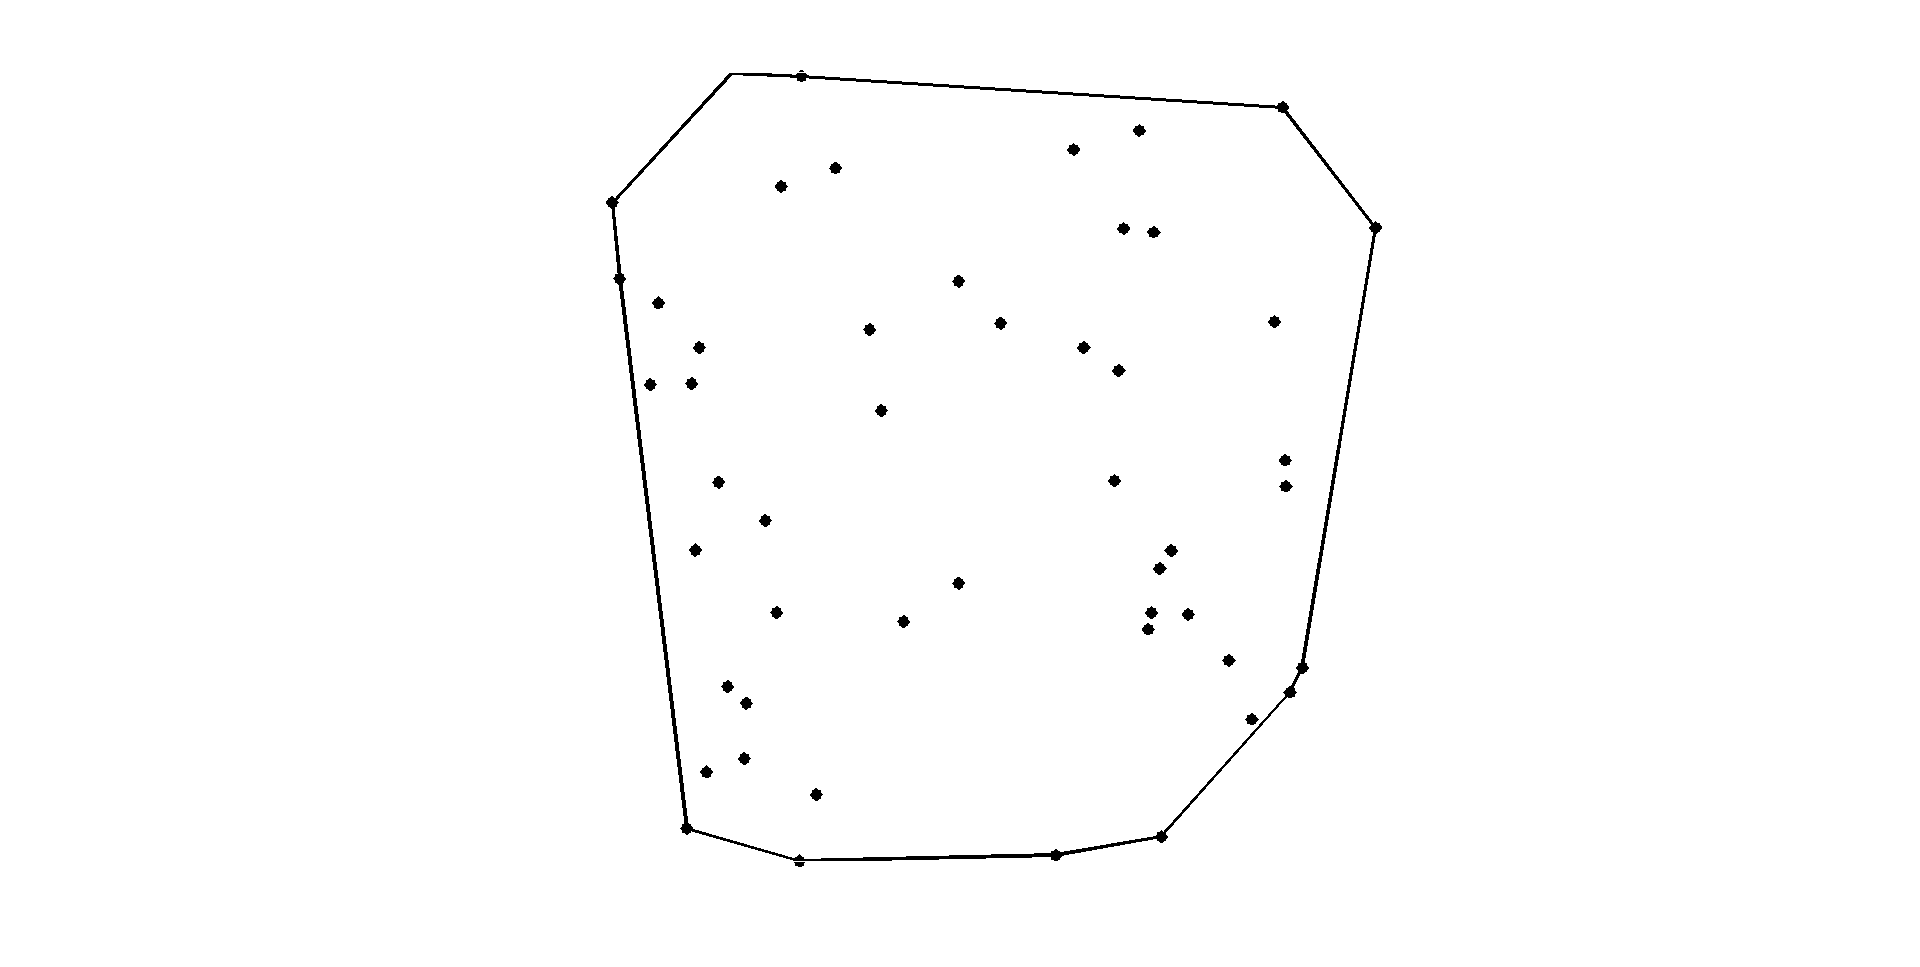
\includegraphics[width=10cm]{convhull.png}%
\end{figure}

\section{Graham scan}
The Graham scan is a method of computing the convex hull of a finite set of points in the plane with time complexity $O(n \log n)$, $n$ is the number of points. It is an evolution of the Gift wrapping algorithm ($O(nh)$, $h$ is the number of points in the hull) in the sense that it avoids evaluating all pairs of angles by first sorting the points.


\subsection{Lowest y-coordinate point}
The first step, as in the gift wrapping algorithm, is to find the point with the lowest y-coordinate. If two points exist in the set, choose the one with the lowest $x$-coordinate: it is denoted $P$. This step obviously takes $O(n)$.

\begin{mcomment}
\begin{mremark}
Use the \minline{min} function.
\end{mremark}
\end{mcomment}

\begin{pcomment}
\begin{premark}
Use the \pinline{numpy.lexsort} function.
\end{premark}
\end{pcomment}

\subsection{Sort by angle}
Next, the set of points must be sorted in increasing order of the angle they and the point $P$ make with the $x$-axis. 


\begin{pcomment}
\begin{premark}
Use the  \pinline{numpy.argsort} function.
\end{premark}
\end{pcomment}

This is the limiting step, it takes $O(n \log n)$. Notice that the cosine of the angle is a decreasing function between 0 and 180 degrees, and will thus avoid to evaluate the angle itself. The sorted set of points is denoted $\mathcal{S}$ (it does not contain $P$).


\subsection{Check angles: left or right turn?}

From the star-like shape issued from the sorting algorithm, construct a list $\mathcal{L}$ of points as: $\mathcal{L}=\{ P, \mathcal{S}, P\}$.

Then, for each triplet of consecutive points $(P_i, P_{i+1}, P_{i+2})$ of $\mathcal{L}$, check if the angle $\widehat{P_i P_{i+1}P_{i+2}}$ is a right turn or a left turn. In case of a right turn, remove $P_{i+1}$ from the list $\mathcal{L}$. Process the entire list this way.



\subsection{Left or right turn?}
Again, determining whether three points constitute a ``left turn'' or a ``right turn'' does not require computing the actual angle between the two line segments, and can actually be achieved with simple arithmetic only. Consider  the cross product of the vectors $\overrightarrow{ P_i P_{i+1}}$ and $\overrightarrow{P_iP_{i+2}}$.

{\SetCustomAlgoRuledWidth{0pt}
\begin{algorithm}[H]
\SetKwProg{myproc}{Procedure}{}{}
 \SetKwFunction{ccw}{ccw} %{$p_1,p_2,p_3$}
 \myproc{\ccw{$p_1,p_2,p_3$}} {
  \KwRet $(p_2.x - p_1.x)*(p_3.y - p_1.y) - (p_2.y - p_1.y)*(p_3.x - p_1.x)$ \;
 }
\end{algorithm}
}

Three points are a counter-clockwise turn if $ccw > 0$, clockwise if $ccw < 0$, and collinear if $ccw = 0$ because $ccw$ is a determinant that gives the signed area of the triangle formed by $p_1$, $p_2$ and $p_3$.

    
\subsection{Convex hull algorithm}
This pseudo-code shows a different version of the algorithm, where points in the hull are pushed into a new list instead of removed from $\mathcal{L}$.

{\SetCustomAlgoRuledWidth{0pt}
\begin{algorithm}[H]
 \KwData{$n$: number of points}
 \KwData{$\mathcal{L}$: sorted list of $n+1$ elements}
 \KwData{First and last elements are the starting point $P$.}
 \KwData{All other points are sorted by polar angle with $P$.}
\SetKwFunction{ccw}{ccw} 
 \CommentSty{stack will denote a stack structure, with push and pop functions.}\\
	\KwData{stack.push($\mathcal{L}(1)$)}
	\KwData{stack.push($\mathcal{L}(2)$)}
	
	\For{$i = 3$ to $n+1$}{
		\While{stack.size$\geq 2$ AND \ccw{stack.secondlast, stack.last, 
		$\mathcal{L}(i)$) $< 0$}}{
			stack.pop();
		}
		stack.push($\mathcal{L}(i)$);
	}
\end{algorithm}
}

In this pseudo-code, stack.secondlast is the point just before the last one in the stack. When coding this algorithm, you might encounter problems with floating points operations (collinearity or equality check might be a problem).


\begin{qbox}
\begin{enumerate}
	\item Generate a set of random points.
	\item Implement and apply the algorithm, and visualize the result.
\end{enumerate}

\end{qbox}
